\documentclass[12pt]{article}
\usepackage[margin=1in]{geometry}
\usepackage{graphicx}
\usepackage{natbib}
\usepackage{hyperref}
\usepackage{url}
\usepackage{amsmath}
\usepackage{booktabs}
\usepackage{subcaption}
\usepackage{float}
\usepackage[most]{tcolorbox}
\usepackage[table]{xcolor}

\definecolor{claudebg}{RGB}{250,235,225}
\definecolor{gptbg}{RGB}{225,235,250}
\definecolor{owbg}{RGB}{235,240,230}

\title{Agent trajectories as programs: procedural fingerprint rollouts}
\author{Hamidah Oderinwale}
\date{May 2026}

\begin{document}
\maketitle

\section{Abstract}
Benchmark scores tell you what an agent got right; they do not tell you how it got there. In this work, we introduce methods for comparing agents procedurally in different contexts, where the model, tasks, and approaches vary. We apply this to evaluation datasets to study how structurally distinct tasks are (at a semantic and syntactic level), and how differently agents approach the same ones. Among benchmarks, we find that procedural complexity across tasks is heavy-tailed. This matters as models saturate existing evals and questions arise about which are most valuable to develop further~\cite{kiela-etal-2021-dynabench}. We find that approaches are linked to model family, that structural similarity follows a long-tail distribution, and that structural representations carry signal not captured by natural language alone. We introduce \texttt{procgrep}, a library for auditing and evaluating agents for how they approach tasks at a procedural level given their traces in a top-down fashion. We believe this work has a range of applications to help developers work with and program coding agents, such as task-aware model routing, agent monitoring, and finer-grained cost analysis.

\section{Introduction}
As programming becomes more high-level, program analysis needs to adapt beyond the syntax level to accommodate agents who can not only be optimized by the code they write but the actions they take. Improving agents will depend on procedural programmability and minimizing the gap between human intent and agent action. Additionally, it will involve assessing trajectories and holistic evaluations beyond binary outcomes \cite{haupt2025position}.

While chain-of-thought has proven itself (eliciting rationale from the agent) useful for post-hoc rationalizing---they cannot be taken as grounded accounts of action \cite{wei2023chainofthoughtpromptingelicitsreasoning, ross2025modelingstudentlearning38, guan2025monitoringmonitorability}. Given this, in this work we explore representations from traces to turn them into structured objects and motivate the need for doing so, and we employ our suite of analytical tools to study the different trajectories that agents take outside controlled settings (in an area of work we call \emph{behavioral fingerprinting}). The goal is to expand the evaluation of agents beyond whether they simply pass or fail a task by venturing into the analysis of their procedural habits or ``style'' \cite{bisztray2025iknowllmwrote}. Additionally, we propose a number of interfaces and measurement frameworks to make these kinds of studies more accessible. Here is where introducing ProcGrep makes sense.

\section{Background}
As agent-style programming becomes more accessible, engineers will spend less time writing code directly and more time shaping how their agents frame and solve problems in the form of \emph{scaffolds}---the wrappers around models that determine which tools they can employ, how they acquire context, and how they react to feedback. That said, traditional program analysis methods are too static to support this reliably and at scale \cite{jimenez2024swebenchlanguagemodelsresolve, yang2024sweagentagentcomputerinterfacesenable, chen2021evaluatinglargelanguagemodels, austin2021programsynthesislargelanguage}. In this work, we introduce a suite of procedural programming tools and analyses on agent traces from software engineering evaluations to address this problem. We motivate this work by showing how variation in agent behavior affects outcomes. While traces can be interpreted in isolation, there is much to gain from studying them in aggregate---tapping into collective wisdom \cite{surowiecki2004wisdom, Alizadeh_2015}---yet there is a lack of tools for doing so, as meaningful comparison calls for shared representations.

Previous work has explored solution variation at scale for MOOCs (massively online open courses) to observe behavior with clustering \cite{glassman2015overcode}. Platforms like LMArena compare agent outputs by evaluating prefered outputs in a pairwise fashion \cite{chiang2024chatbotarenaopenplatform}. Prior work has investigated using LLMs to generate plans from formal specifications~\cite{silver2024generalized}; with procedural representations it is possible to do the inverse, where queries can be written as procedural specs to `grep' traces.~\cite{yin2017syntacticneuralmodelgeneralpurpose}. Observational studies of LLM chats have been performed at scale to understand trends in model use \cite{tamkin2024clioprivacypreservinginsightsrealworld, deming2025how}. Frameworks have also been introduced for configuring models as agents to perform multi-step tasks with their own feedback loops given a goal specified upfront with `discovered' end states \cite{yao2023reactsynergizingreasoningacting}. And past work has also shown that coding style can be derived from source code using ASTs and decision trees in the form of random forest classifiers \cite{code_stylometry}. \textcolor{blue}{Most closely related, code stylometry attributes LLM-generated \emph{source} to its author model---up to 97.56\% binary and 95.40\% five-way over 32k generated C programs \cite{bisztray2025iknowllmwrote}. That work fingerprints the \emph{artifact} (the code produced); we fingerprint the \emph{process} (the trajectory of actions), capturing intra-trajectory structure---phase transitions, conditional decision logic, lineage drift---that output stylometry cannot see.}

Existing frameworks have been built for code alone in siloed environments where context is missing, looking at patches \cite{GumTree2014, yin-neubig-2017-syntactic} with ASTs (abstract syntax trees) which generalizes across languages. We make use of established parsing methods and extend them to work in multi-modal free-form environments where prompts, for example, are written in natural language \cite{cruz2026textastherichestpreferencesignal} demonstrating that a rich set of features can be observed and made sense of. Next, given one's ability to audit procedures, there is an avenue for work which involves seeing what processes yield the best outputs. A new kind of model routing adapted to preferences could blossom from this direction. We explore it lightly in this work.

\section{A theory of procedural understanding}
Framing agent coding traces as procedures lets us comparatively study and interact with them in ways that are useful for benchmarking, evaluating the difficulty of evals themselves, differentiating models by their behavioral fingerprints, and performing procedural search. We release a library called ProcGrep to support these use cases. For example, ProcGrep supports queries such as the following.

\begin{tcolorbox}[colback=black!3, colframe=black!30, boxrule=0.4pt, left=10pt, right=10pt, top=8pt, bottom=8pt, fontupper=\small]
All Claude-4 trajectories from the past two weeks on Python repositories where \texttt{search\_repo} was followed by three or more \texttt{read\_file} calls within the first 8 steps, the agent then made at least one edit, and no \texttt{run\_test} occurred before the final submit---on instances with difficulty score above 3.
\end{tcolorbox}

In this work, we use traces for a number of popular software engineering benchmarks and test a number of SOTA model families (GPT, Claude, DeepSeek, and Qwen). We use public archives of model traces for SWE-Bench (\url{princeton-nlp/SWE-bench-experiments}) and do the same for Agentless logs. \textcolor{blue}{Table~\ref{tab:models} lists the full set of agents studied: ten agents across four scaffolds (SWE-agent, Agentless, DARS, Moatless) spanning the GPT, Claude, DeepSeek, and Qwen families.}

\begin{table}[H]
\centering\small
\begin{tabular}{lllr}
\toprule
\textbf{Scaffold} & \textbf{Model} & \textbf{Paradigm} & \textbf{$n$} \\
\midrule
\rowcolor{claudebg} SWE-agent & Claude-3 Opus        & RLHF dense        & 300 \\
\rowcolor{claudebg} SWE-agent & Claude-3.5           & RLHF dense        & 289 \\
\rowcolor{claudebg} SWE-agent & Claude-3.7 (thinking)& Extended thinking & 284 \\
\rowcolor{claudebg} SWE-agent & Claude-4             & Extended thinking & 288 \\
\rowcolor{gptbg}    SWE-agent & GPT-4                & RLHF dense        & 300 \\
\rowcolor{gptbg}    SWE-agent & GPT-4o               & RLHF dense        & 278 \\
\rowcolor{owbg}     DARS      & DeepSeek-R1          & RL reasoning      & 300 \\
\rowcolor{owbg}     Agentless & Claude-3.5           & RLHF dense        & 300 \\
\rowcolor{owbg}     Moatless  & DeepSeek-V3          & MoE pretrain      & 300 \\
\rowcolor{owbg}     SWE-agent & SWE-agent-LM-32B$^\dagger$ & SFT-distilled (Qwen2.5-32B) & 498 \\
\bottomrule
\end{tabular}
\caption{\textcolor{blue}{Models and scaffolds studied (ten agents). $^\dagger$Distilled from the Claude-3.7 teacher (row 3); analysed in \S\ref{sec:distillation}.}}
\label{tab:models}
\end{table}

We define what is the appropriate language to describe and program their behavior. What we call a ``procedural fingerprint'' is recovered from what an agent actually did (its trajectory) rather than its components or what it states. A fingerprint is a distinguishable feature of an agent from other agents and is consistent over time.

\textcolor{blue}{Firstly, we demonstrate that these fingerprints exist: a logistic-regression probe over procedures identifies which of nine agents produced a trajectory at \textbf{85.7\%} accuracy (macro-F1 0.85), versus an 11.1\% random baseline ($\approx$ chance for nine classes)---a $7.7\times$ lift we attribute to problem-solving \emph{style}. The probe is leakage-controlled: under GroupKFold by task (no instance shared between train and test) accuracy is essentially unchanged from standard cross-validation (leakage $\Delta = -0.007$), so the signal is style, not task memorization. Identifiability is uneven (Table~\ref{tab:attribution}). Deterministic scaffolds are near-perfectly identifiable (Agentless and DARS F1 $=$ 1.00, Moatless 0.97), as expected. Among models sharing the SWE-agent scaffold, the \emph{extended-thinking} models are the most distinctive (Claude-4 and Claude-3.7-thinking, F1 $=$ 0.99), while the older RLHF-dense models are the most confusable (GPT-4 0.62, Claude-3 0.65, GPT-4o 0.65)---still 5--6$\times$ chance. The thinking models' orchestration style leaves a sharper procedural trace than the more generic dense-model workflow. This attribution is leakage-controlled at the step level: we name the agent on a task we have never seen it solve. The scope is closed-set over nine known agents (leaderboard submissions); open-world attribution of undisclosed models is left to future work.}

\begin{table}[H]
\centering\small
\begin{tabular}{lr}
\toprule
\textbf{Agent} & \textbf{F1} \\
\midrule
\rowcolor{owbg}     Agentless+Claude-3.5 & 1.00 \\
\rowcolor{owbg}     DARS+DeepSeek-R1     & 1.00 \\
\rowcolor{claudebg} Claude-3.7-thinking  & 0.99 \\
\rowcolor{claudebg} Claude-4             & 0.99 \\
\rowcolor{owbg}     Moatless+DeepSeek-V3 & 0.97 \\
\rowcolor{claudebg} Claude-3.5           & 0.82 \\
\rowcolor{gptbg}    GPT-4o               & 0.65 \\
\rowcolor{claudebg} Claude-3             & 0.65 \\
\rowcolor{gptbg}    GPT-4                & 0.62 \\
\bottomrule
\end{tabular}
\caption{\textcolor{blue}{Per-agent identification F1 from the nine-way probe (LogisticRegression over TF-IDF of BPE procedures; GroupKFold by task). Overall accuracy 85.7\% vs.\ 11.1\% chance. Scaffolds and extended-thinking models are near-perfectly identifiable; older dense models are the most confusable.}}
\label{tab:attribution}
\end{table}

\textcolor{blue}{The attribution task is set up as follows. We take every trajectory from the nine agents, canonicalize each into an action sequence and merge it into recurring procedures (\S\ref{sec:vocab}), and treat each trajectory's procedure sequence as a document. We vectorize with TF-IDF (so procedures common to all agents are down-weighted and distinctive ones up-weighted), label each document with its producing agent, and fit a linear classifier, evaluating out-of-fold under GroupKFold grouped by task instance.}

First, we consider a distilled model pair, where there is a teacher and student model\textcolor{blue}{ (the full case study is in \S\ref{sec:distillation})}. \textcolor{blue}{Distillation lowers cost-per-task, but does it transfer the teacher's decision structure or only surface behavior? This is the question \S\ref{sec:distillation} takes up.}

Given a set of procedures that we might want to compare, which we can call a procedural space, we need a vocabulary or a set of actions that we can use to describe all of them. The contributions of this framework comes from being able to define this vocabulary bottom-up instead of with a more hard-coded or classifier based approach. We benchmark our methods against prompt-based classifiers, finding that \textcolor{blue}{across four judge models, prompt-based classifiers label 17--38\% of instances as compositionally divergent with near-zero cross-family agreement ($\kappa < 0.05$), demonstrating that natural-language descriptions of procedural divergence are unstable}. This affirms our motivations for having representations that can be shared across models and instances to allow for comparative analysis.

\textcolor{blue}{A prompt-based classifier (GPT-4o as judge) labels 38\% of instance pairs as compositionally divergent, with agreement dropping to near zero across model families ($\kappa < 0.05$); see Table~\ref{tab:divergence_by_model} in the Appendix. This instability motivates the structural vocabulary below.} This means that there are features of the full vocabulary or alphabet which we can study in itself and can form the basis of insights. To define our vocabulary, we need to be able to extract these procedures and label them to understand what they are. Each procedure should be composable and collapse into one another because steps are taken in sequence for specific tasks and to avoid redundancy---where each procedure of the trajectory should be meaningfully unique or composed of unique sub-procedures.

\textcolor{blue}{The induced vocabularies differ in size by nearly two orders of magnitude, and this span is itself a procedural-diversity signal. Repertoire@90\%---the number of distinct procedures needed to cover 90\% of an agent's actions (Table~\ref{tab:per-agent-megatable})---ranges from 1 for Agentless, which collapses to a single repeated procedure (entropy 0.00), to 49 for GPT-4o. Deterministic and constrained scaffolds sit at the low end (Agentless 1, Moatless 12, DARS 19) while open-ended model-driven agents spread widely (GPT-4o 49, Claude-3 Opus 44, GPT-4 40); the extended-thinking models are mid-pack (Claude-3.7 32, Claude-4 35) despite the highest resolve rates. Procedural diversity therefore tracks how much the scaffold constrains behavior, not model capability.}

\subsection{Vocabulary induction}
\label{sec:vocab}
BPE or Byte-Pair Encoding is a useful analog for this process. While BPE chunks natural language tokens by merging those that frequently appear together to compress the data for pre-training LLMs, we chunk actions from generated code \cite{sennrich2016neuralmachinetranslationrare}. \textcolor{blue}{The idea of learning a compact vocabulary bottom-up from procedural traces connects to program synthesis work on library learning~\cite{ellis2020dreamcodergrowinggeneralizableinterpretable}, where recurring program fragments are abstracted into reusable procedures; here the corpus drives vocabulary induction rather than a task-specific objective.} Like BPE, our vocabulary is learned or derived from the procedures themselves rather than hand-specified, and when a procedure is added to the vocabulary it is now a meaningful member of an alphabet. With BPE, however, there is no dynamic stopping point for the algorithm which means that a target vocabulary size needs to be set up front.

\textcolor{purple}{TODO: trace\_pipeline.png not yet produced --- figure commented out below until the illustration is made.}
%\begin{figure}[H]
%    \centering
%    \includegraphics[width=1\linewidth]{figures/trace_pipeline.png}
%    \caption{Illustrative figure of the process of vocabulary induction given an agent trace.}
%    \label{fig:encoding_pipeline}
%\end{figure}

We consider the induction of a vocabulary to be a similar class of problem to a clustering one, so we draw on how clustering algorithms are evaluated to form the basis of an emergent stopping criterion \cite{rosenberg-hirschberg-2007-v}. We use the V-measure as our evaluation for the mined procedures. We consider a vocabulary stable when it maximizes two measures: completeness, meaning the sub-actions of each procedure are correctly aligned with an intent, and homogeneity, meaning a procedure contains only actions that belong to it.

\[ V = 2 \cdot \frac{h \cdot c}{h + c} \]
where homogeneity $h$ and completeness $c$ are defined as
\[ h = 1 - \frac{H(\text{actions} \mid \text{procedure})}{H(\text{actions})} \qquad c = 1 - \frac{H(\text{procedure} \mid \text{actions})}{H(\text{procedure})} \]
$H(\text{actions} \mid \text{procedure})$ measures the confidence of belonging of an action to a procedure, and $H(\text{procedure} \mid \text{actions})$ measures the reverse. A vocabulary is stable when $V$ is maximized.

To extract the actions themselves, we take code hunks---solution patches---from these evaluation datasets and then parse them with an AST that gives a node tree and a syntactical and semantic representation of the code. Given the structural representation of the solution patches, we then apply an embedding stage to encode the change in plain language and the underlying intent by contextualizing the structured patch with the surrounding code and a behavioral description from the model.

\textcolor{blue}{Another property of the optimal vocabulary is that the procedures it contains are distinguishable and non-redundant. We compare BPE against PrefixSpan, the standard sequential-pattern miner, by clustering trajectories under each vocabulary and scoring the clusters against agent labels (Figure~\ref{fig:bpe_vs_prefixspan}): at matched procedure count BPE reaches V-measure 0.606 ($K=64$, rising to 0.626 at $V=128$) versus 0.505 for PrefixSpan. BPE's hierarchical merging builds more agent-discriminative procedures than the flat set produced by PrefixSpan.}

We investigate entropy within the context of a collective with Jensen-Shannon Divergence. Entropy (H), a measure of uncertainty in a distribution (where a distribution here is the probability over all the possible actions in our vocabulary), is a property that can be applied to a single agent's distribution of actions, where it is defined as: $$H(a) = -\sum_{v \in \mathcal{V}} p_a(v) \log_2 p_a(v)$$ JSD allows us to build on entropy and measure how different two distributions are and is defined as: $$\mathrm{JSD}(a, b) = H\!\left(\frac{p_a + p_b}{2}\right) - \frac{1}{2}H(a) - \frac{1}{2}H(b)$$

Across all models, passing behavior includes a higher ratio of browsing to other actions. Extended thinking Claude models spend the largest proportion of their time in the shell compared to older models with more even task breakdowns. Models in the GPT family have more consistent behavior, but newer ones spend more time editing. Agent harnesses have less task diversity, potentially due to their programmed behavior and have more distinct breakdowns, the Agentless scaffold spends a disproportionate amount of time browsing and the Moatless scaffold leads to a large proportion of testing. An interesting application of this is forecasting the costs of an agent, as it is not only a product of the cost per tool call, but a function of the action types needed to complete it and the procedural tendencies of the model being orchestrated.

\begin{figure}[H]
    \centering
    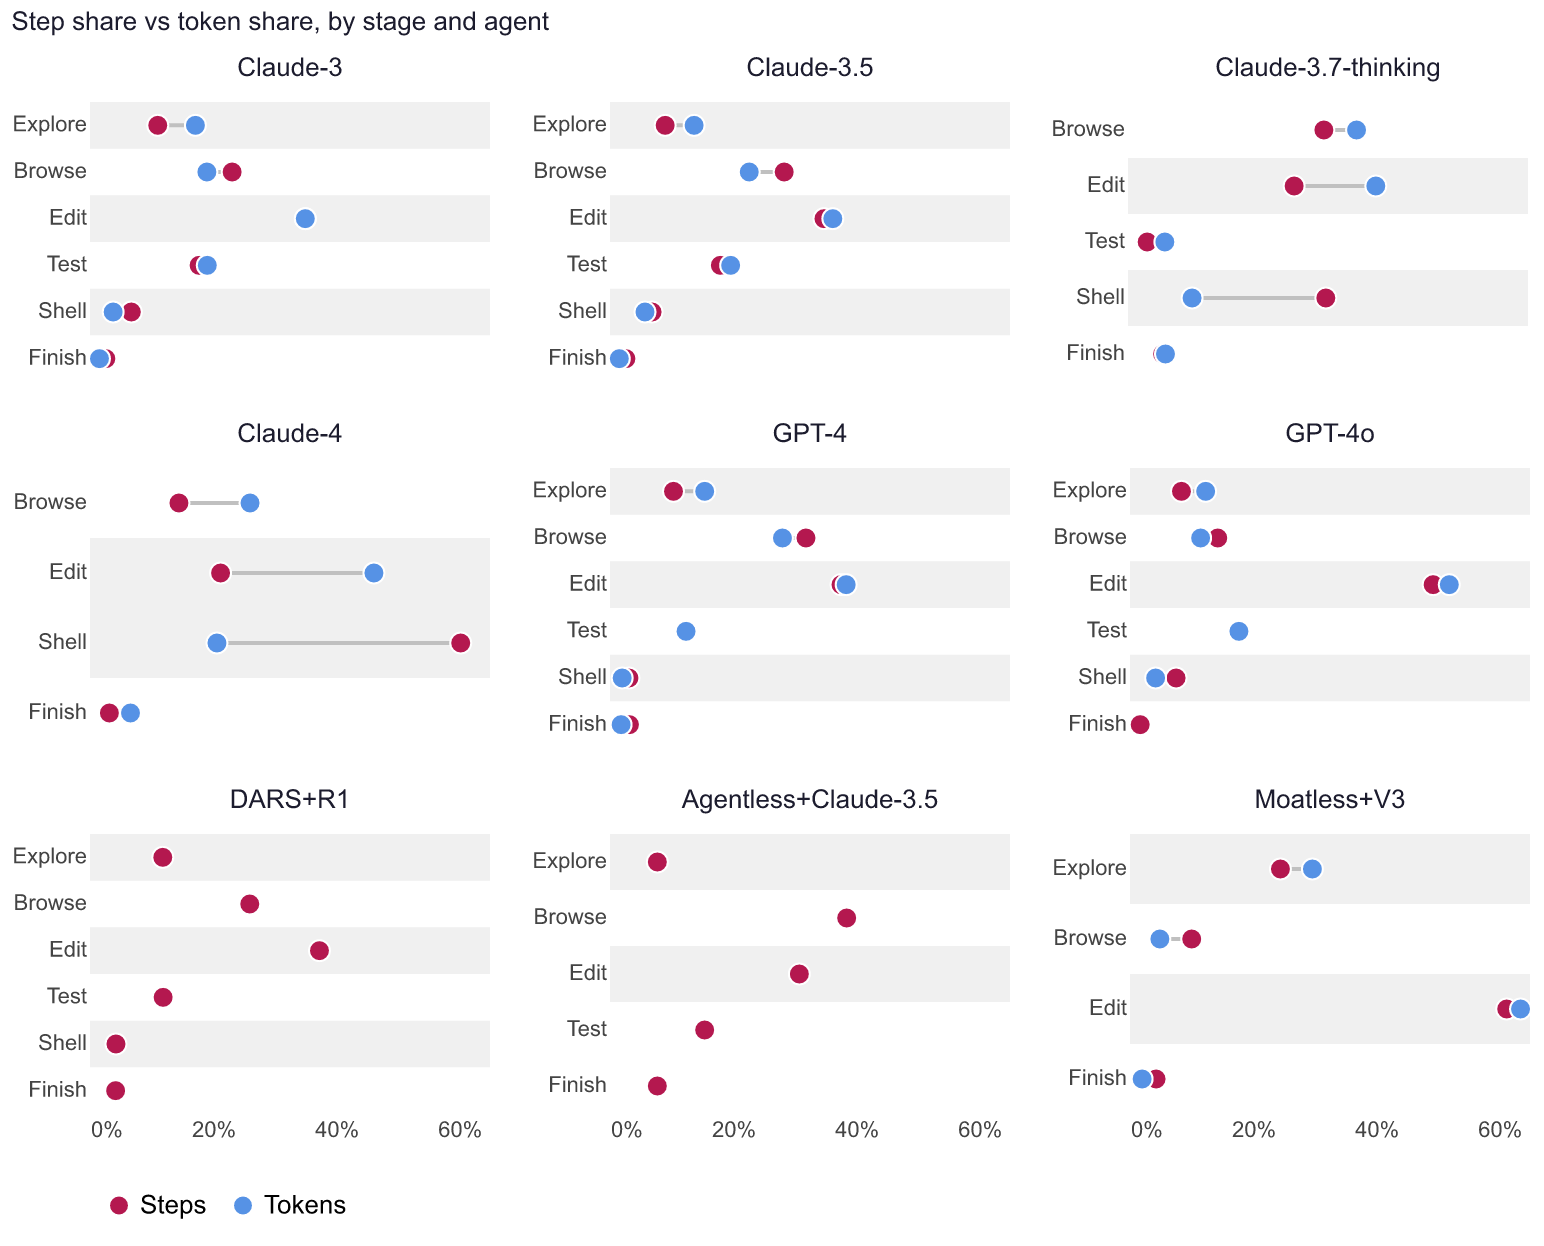
\includegraphics[width=0.82\linewidth]{figures/fig_step_vs_token_cost.png}
    \caption{Cost breakdown of agents by action type and tokens.}
    \label{fig:step_token_cost}
\end{figure}

\begin{figure}[H]
    \centering
    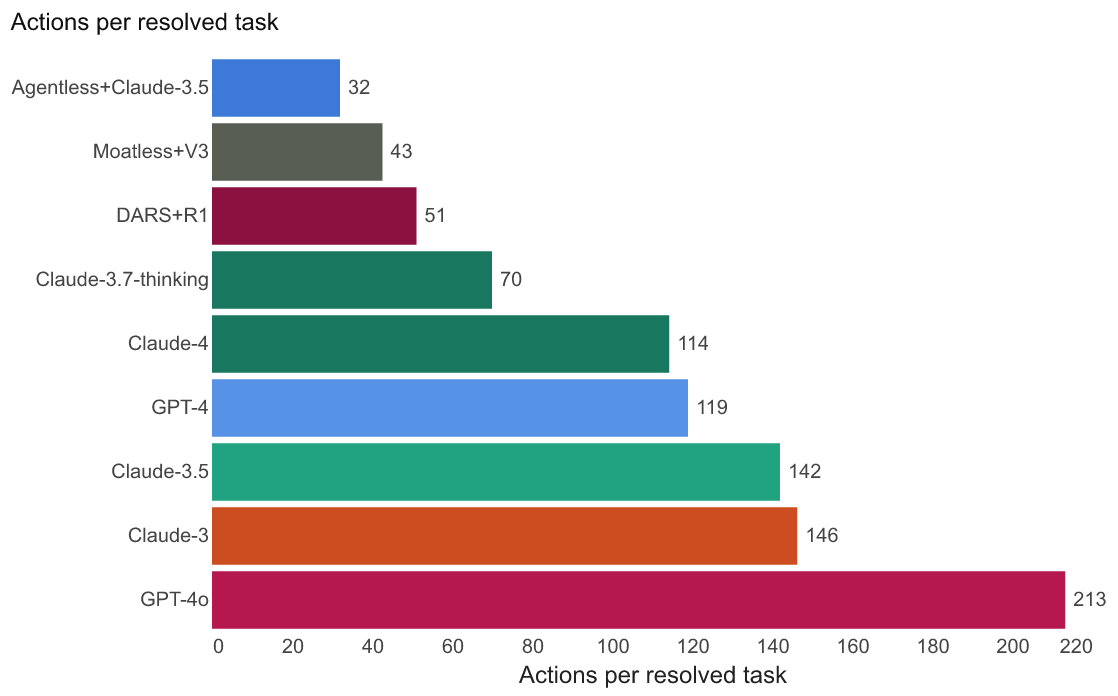
\includegraphics[width=0.5\linewidth]{figures/fig_steps_per_resolved.png}
    \caption{Average number of steps per resolved tasks across agents.}
    \label{fig:steps_resolved}
\end{figure}

\begin{table*}[H]
\centering\footnotesize\setlength{\tabcolsep}{4pt}
\resizebox{\linewidth}{!}{%
\begin{tabular}{lllrrrrrrrrr}
\toprule
\textbf{Scaffold} & \textbf{Model} & \textbf{Paradigm} & \textbf{$n$} & \textbf{Resolve} & \textbf{Steps} & \textbf{Repertoire} & \textbf{Compr.} & \textbf{Entropy} & \textbf{Cost/task} & \textbf{\$/step} & \textbf{Cost/resolved} \\
 & & & & & \textbf{/traj} & \textbf{@90\%} & \textbf{ratio} & \textbf{(bits)} & & & \\
\midrule
\rowcolor{claudebg} SWE-agent & Claude-3 Opus & RLHF dense & 300 & 11.7\% & 17.1 & 44 & 0.537 & 5.58 & \$3.42 & \$0.200 & \$29.31 \\
\rowcolor{claudebg} SWE-agent & Claude-3.5 & RLHF dense & 289 & 23.9\% & 32.7 & 42 & 0.559 & 5.56 & \$1.62 & \$0.050 & \textcolor{blue}{\$7.06} \\
\rowcolor{claudebg} SWE-agent & Claude-3.7-thinking & Extended thinking & 284 & 50.7\% & 33.6 & 32 & 0.471 & 5.14 & \$0.78 & \$0.023 & \$1.53 \\
\rowcolor{claudebg} SWE-agent & Claude-4 & Extended thinking & 288 & 59.0\% & \textbf{64.8} & 35 & 0.417 & 5.26 & \$1.19 & \$0.018 & \$2.02 \\
\midrule
\rowcolor{gptbg} SWE-agent & GPT-4 & RLHF dense & 300 & 18.0\% & 21.4 & 40 & 0.443 & 5.47 & \$2.51 & \$0.117 & \$13.93 \\
\rowcolor{gptbg} SWE-agent & GPT-4o & RLHF dense & 278 & 19.8\% & 39.1 & \textbf{49} & 0.425 & 5.76 & \$2.53 & \$0.065 & \textcolor{blue}{\$13.82} \\
\midrule
\rowcolor{owbg} DARS & DeepSeek-R1 & RL reasoning & 300 & 47.0\% & 24.0 & 19 & \textbf{0.572} & 4.44 & \$2.43$^*$ & --- & \$5.17$^*$ \\
\rowcolor{owbg} Agentless & Claude-3.5 & RLHF dense & 300 & 40.7\% & 13.0 & \textbf{1} & \textbf{0.077} & \textbf{0.00} & \$0.50$^*$ & --- & \$1.23$^*$ \\
\rowcolor{owbg} Moatless & DeepSeek-V3 & MoE pretrain & 300 & 30.7\% & 13.1 & 12 & 0.417 & 3.71 & \$0.02 & ${\approx}0$ & \$0.06 \\
\bottomrule
\end{tabular}%
}
\\[0.3em]
{\footnotesize $^*$Cost estimated. \$/step = cost per inference call. Extended thinking models reduce cost per step by routing calls through the shell and orchestrating them before invoking the more expensive inference calls (Claude-4: \$0.018/step vs.\ Claude-3: \$0.200/step).}
\caption{Per-agent procedural fingerprint and cost efficiency on SWE-bench Lite ($n=2{,}639$).}
\label{tab:per-agent-megatable}
\end{table*}

\begin{figure}[H]
    \centering
    
\includegraphics[width=\linewidth]{figures/token_cost_by_difficulty.png}
    \caption{\textcolor{blue}{Input tokens, API calls, and dollar cost per task vs.\ task difficulty (number of agents that solved the task). All three decline monotonically as tasks get easier---cost tracks task difficulty, not just per-call price. The cost panel is restricted to the SWE-agent submissions that report \texttt{info.model\_stats}; newer/open-weight agents lack cost telemetry.}}
    \label{fig:token_cost_difficulty}
\end{figure}

\begin{table}[H]
\centering
\begin{tabular}{lccc}
\toprule
\textbf{Representation} & \textbf{n} & \textbf{F1 (k=1)} & \textbf{Source} \\
\midrule
Structural pattern overlap  & 289 & 0.347 & Deterministic \\
Action sequence distance    & 289 & 0.274 & Deterministic \\
Edit action overlap         & 289 & 0.256 & Deterministic \\
Narrative description       & 289 & 0.177 & Varies by model \\
Agent plan description      & 289 & 0.155 & Varies by model \\
Divergence classifier (LLM) & 87--286 & 0.000--0.363 & $\kappa < 0.05$ (cross-family) \\
\midrule
Random retrieval            & 289 & 0.13--0.24 & Baseline \\
\bottomrule
\end{tabular}
\caption{\textcolor{blue}{Pass/fail prediction F1 at the single nearest neighbour ($k{=}1$). \emph{Deterministic}: computed directly from the trace (reproducible); \emph{varies by model}: depends on a model's natural-language account. Structural representations beat the random-retrieval floor (0.13--0.24, the 12--24\% base pass rate) by $+$0.10--0.22; the LLM divergence classifier is unstable across four judges ($\kappa<0.05$).}}
\label{tab:representation_comparison}
\end{table}

\section{Why procedural representations matter}
Given theoretical grounding, we put foundations to work in a number of ways. In this section we look at top-down analyses given agent traces. Firstly, we show that these approaches offer a more grounded representation of process than what can be elicited from models in natural language alone. We ask two questions: given what a model says it will do, what does it actually do (forward coverage)? Then, given what a model says it did, what did it actually do (reverse coverage)? \textcolor{blue}{Forward coverage is high across families, but reverse coverage is not---and it is lowest for the extended-thinking models (Claude-3.7-thinking and Claude-4 reach only $\approx$0.20--0.25 median reverse coverage, versus 0.50--0.71 for the older models, Figure~\ref{fig:cot_alignment}). In other words, thinking models narrate the least of what they actually do: many actions they take are never mentioned in their reasoning.}

\begin{figure}[H]
    \centering
    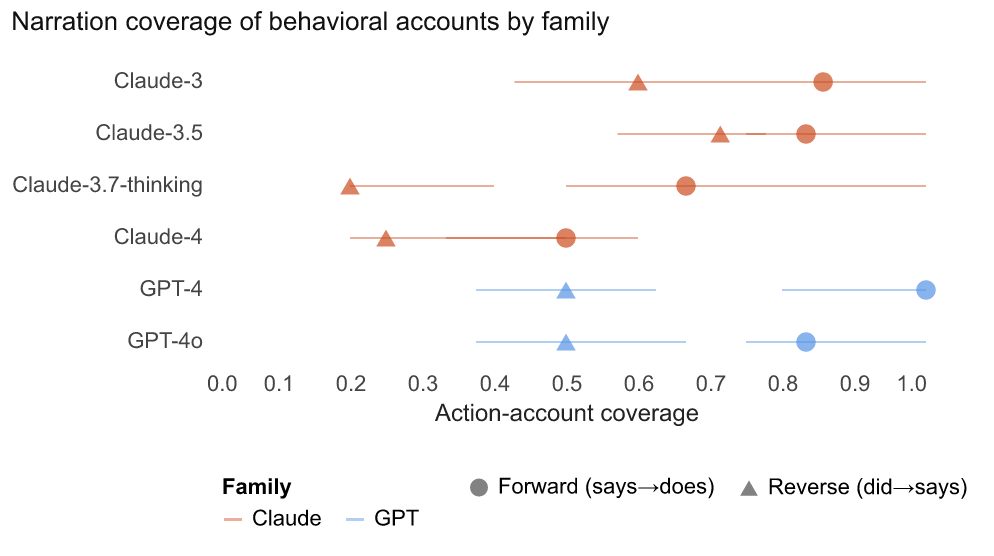
\includegraphics[width=0.6\linewidth]{figures/cot_alignment_6agents.png}
    \caption{\textcolor{blue}{Narration coverage of behavioral accounts by family: forward coverage (says$\to$does) and reverse coverage (did$\to$says) per agent, with IQR. Forward $\gg$ reverse everywhere; extended-thinking models have the lowest reverse coverage.}}
    \label{fig:cot_alignment}
\end{figure}

Then, we consider precision in the behavioral descriptions themselves. We find that models are generally verbose in their accounts, which might be a signal of performative chain-of-thought \cite{boppana2026reasoningtheaterdisentanglingmodel}. For example, the GPT family are trained with heavy RLHF and instruction-tuning. Whereas the Claude family of models are presumably trained to follow more sprawling reasoning patterns before coalescing them into some preferred approach. Extended thinking models are the most verbose and have similar behavior to the baseline of shuffled rationales.

\begin{table}[H]
\centering\small
\begin{tabular}{lrrrrr}
\toprule
\textbf{Model} & \textbf{n} & \textbf{Verbosity} & \textbf{Precision} & \textbf{Baseline} & \textbf{Recall} \\
\midrule
\rowcolor{claudebg} Claude-3            & 300 & 1.07 & 0.833 & 0.678 & 0.857 \\
\rowcolor{claudebg} Claude-3.5          & 289 & 1.00 & 0.857 & 0.732 & 0.833 \\
\rowcolor{claudebg} Claude-3.7-thinking & 284 & 1.35 & 0.625 & 0.623 & 0.800 \\
\rowcolor{claudebg} Claude-4            & 288 & 1.32 & 0.500 & 0.536 & 0.750 \\
\midrule
\rowcolor{gptbg}    GPT-4               & 300 & 1.17 & 0.800 & 0.713 & 1.000 \\
\rowcolor{gptbg}    GPT-4o              & 278 & 1.18 & 0.750 & 0.679 & 1.000 \\
\midrule
\rowcolor{owbg} DARS+R1 & 300 & 1.07 & 0.857 & 0.775 & 0.875 \\
\bottomrule
\end{tabular}
\caption{\textcolor{blue}{Behavioral-account precision and recall by model. Verbosity is the ratio of stated to observed actions; baseline is a shuffled-rationale control. Extended-thinking models are the most verbose and least precise.}}
\label{tab:verbosity}
\end{table}

\section{Natural experiments with procedural representations}
With this data, we can also validate other kinds of inferences regarding the shapes of problems and model behavior. For example, past work has found that models struggle with compositional generalization---this means that they are brittle in contexts where they need to do incremental work. We validate this in the wild and find that problems that require compositional generalization, defined by problems that have nested procedures, are especially difficult for agents, as evidenced by their failure rates. We define compositional problems as ones where the subproblems are ones that have been solved by the agent before, but when put together the agent failed. Looking at Figure~\ref{fig:compositional_failure} we can observe that compositionality is a relatively strong signal of failure, followed by novel actions, and familiar procedures yield the lowest failure rates. However, the pattern holds the most strongly for RLHF-trained models and much more modest for more classically trained models. Across models, similar trends hold, but open-weight agents have lower failure rates to compositional problems---When computing the difference of open-weight model failure at all points compared to other model families is ${\sim}9\%$.

Additionally, we look at different agent pipelines and compare them across 289 tasks (Agentless v. SWE-Bench Agent). Agentless successfully solves 63 more tasks than SWE-Agent and we can use the procedural methods for assessing why.

\begin{table}[H]
\centering\small
\begin{tabular}{lrrrr}
\toprule
\textbf{Outcome} & \textbf{$n$} & \textbf{Difficulty} & \textbf{SWE-agent steps} & \textbf{Agentless steps} \\
\midrule
Both pass       &  54 & 7.17 & 20.4 & 13.0 \\
SWE-agent only  &  15 & 4.53 & 30.7 & 13.0 \\
Agentless only  &  63 & 4.59 & 33.3 & 13.0 \\
Neither passes  & 157 & 0.69 & 36.8 & 13.0 \\
\midrule
\multicolumn{2}{l}{Total} & & 289 \\
\bottomrule
\end{tabular}
\caption{Outcomes of two agent scaffolds on 289 tasks.}
\label{tab:scaffold_outcomes}
\end{table}

\begin{figure}[H]
\centering
\begin{subfigure}[t]{0.3\linewidth}
    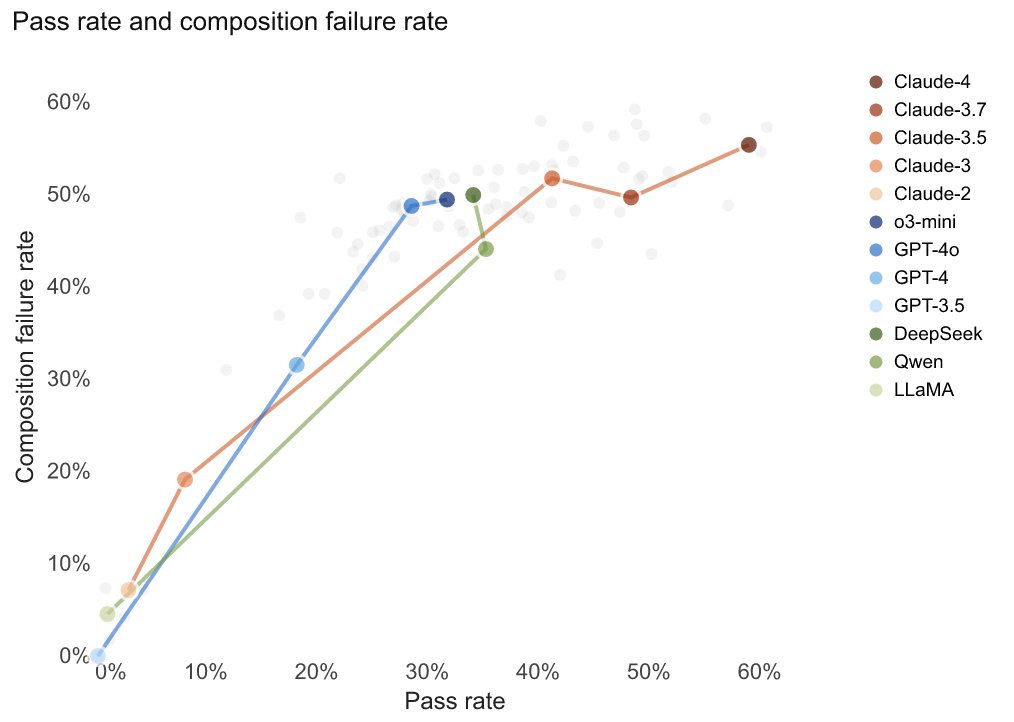
\includegraphics[width=\linewidth]{figures/failure_mix_by_agent_84.png}
    \caption{Relationship between compositional problems and pass rate across models.}
    \label{fig:compositional_failure}
\end{subfigure}
\hfill
\begin{subfigure}[t]{0.6\linewidth}
    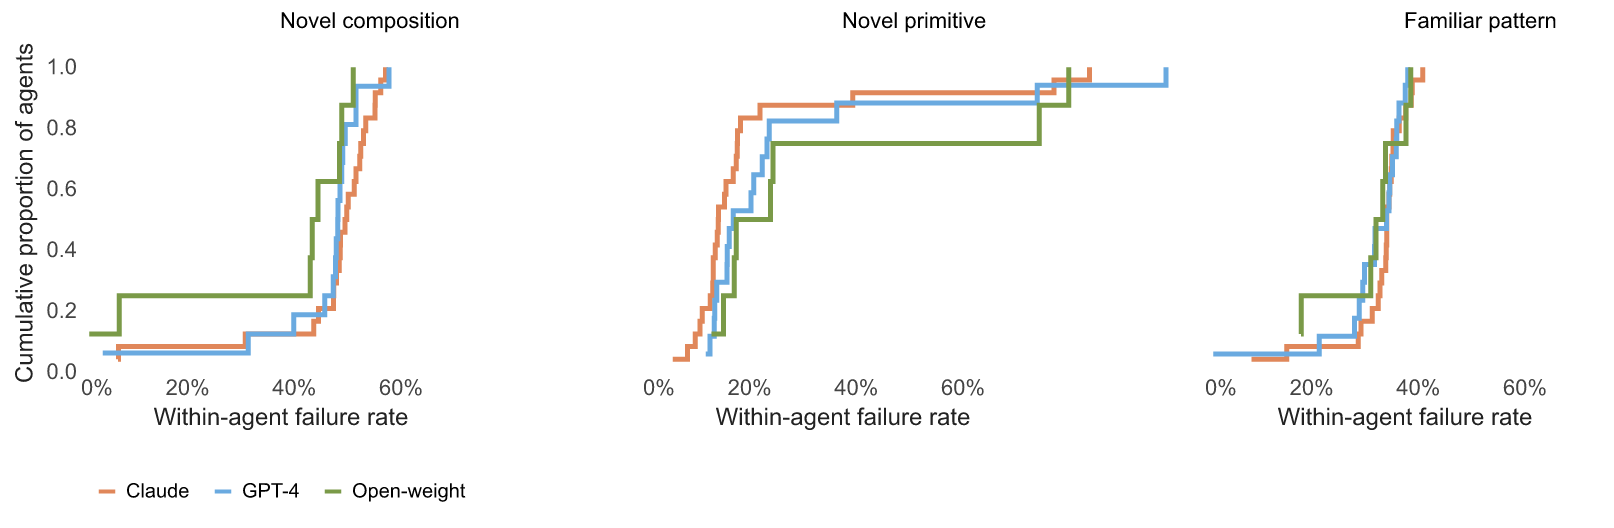
\includegraphics[width=\linewidth]{figures/failure_by_family.png}
    \caption{Failure type distributions by model family.}
    \label{fig:failure_by_family}
\end{subfigure}
\caption{Model behavior on compositional tasks.}
\label{fig:composition_analysis}
\end{figure}

\textcolor{blue}{This raises a sharper question: are procedural styles mere \emph{preferences}, or are they \emph{load-bearing} for capability? The Agentless--SWE-agent comparison is a natural experiment---Agentless forces a localize-first, browse-heavy style on Claude-3.5, and that constraint \emph{raises} resolution from 23.9\% (free SWE-agent) to 40.7\%, suggesting the style is load-bearing rather than cosmetic (with the caveat that the scaffold changes more than style alone). Holding difficulty fixed sharpens it: at \emph{independent} difficulty (leave-the-agent-out solve rate, so an agent's own outcome never enters its own difficulty axis), agent identity barely matters on easy or hard tasks but spans 11--89\% at medium difficulty (Figure~\ref{fig:agent_by_difficulty}), and Claude-4 is the only agent with appreciable hard-task capability (33\% vs.\ $\le$17\%). A clean causal test---constraining a model's own preferred style at a fixed token budget and measuring the change in capability---requires controlled intervention runs and is left to future work.}

\begin{figure}[H]
    \centering
    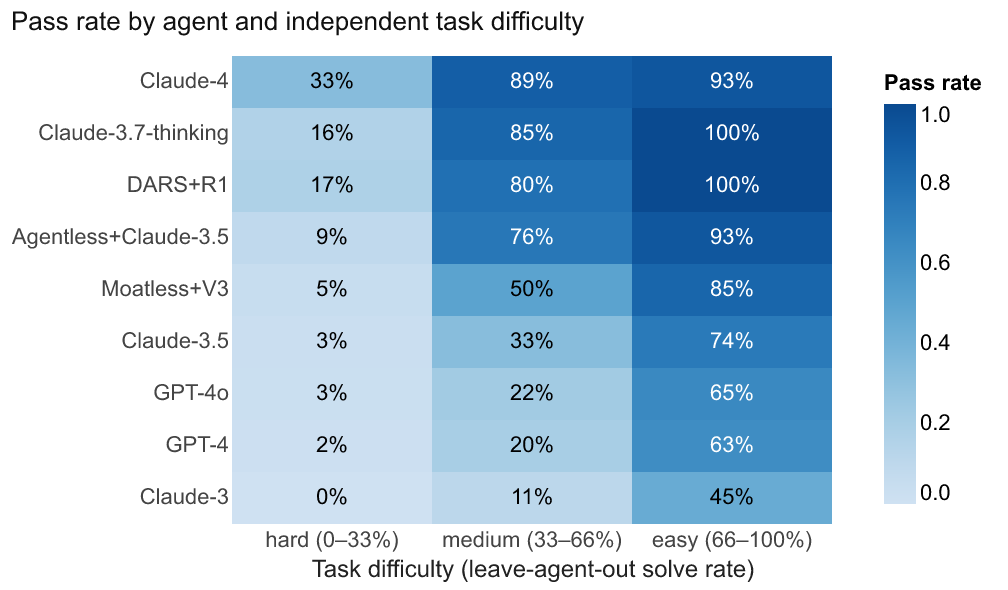
\includegraphics[width=0.68\linewidth]{figures/fig_agent_by_difficulty.png}
    \caption{\textcolor{blue}{Pass rate by agent and \emph{independent} task difficulty (leave-the-agent-out solve rate). Agent identity matters most at medium difficulty (spread 11--89\%) and converges at the extremes; among models the extended-thinking ones (Claude-4, Claude-3.7) lead and Claude-4 alone has appreciable hard-task capability.}}
    \label{fig:agent_by_difficulty}
\end{figure}

Next, developers make a number of decisions to train and scaffold their models. We set out to understand how this affects model processes based on a set of tasks and find that ``fingerprints'' are recoverable---unique model-specific patterns regarding tool-use and order of operations. Given certain parameters like the costs for different types of actions and the length of a task, hopefully this can form the basis of more informed model choice and configuration decisions depending on a developer's goal (i.e.\ task and workflow-aware routing). For a given model, its procedural space can be described by its entropy and compression, where entropy describes the variance of the actions and compression is a rough proxy for repetitiveness. We find the GPT-4o has the most diversity of actions compared to Claude models.

\textcolor{blue}{Fingerprints also surface exploration style. Claude-3.5 opens the most files per trace (mean 2.41 vs.\ 1.66--1.90 for peers) and degrades the least when spreading across multiple files: pass rate drops from 29.0\% (1 file) to 17.6\% (3+ files), compared to GPT-4o's 27.3\%~$\to$~8.1\%. Claude-3.5 spreads wider and degrades less for doing so.}

\subsection{In-task monitoring}
\textcolor{blue}{Because procedural patterns form as a trajectory runs, failure is detectable while the agent is still working---enabling early-abort and escalation rather than only post-hoc analysis. We train a logistic-regression probe on the first $k$ canonical actions to predict eventual resolution, leakage-controlled with GroupKFold by task. Failure is already separable from the first three actions (AUC 0.69) and rises only modestly to 0.72 by step 20 (Table~\ref{tab:early_abort_auc}); this is procedural signal rather than length, since resolved and unresolved trajectories have near-identical median length (19 vs.\ 20 steps). Re-scoring the prefix at every step and aborting the first time $P(\text{resolve})<\tau$ (no fixed decision step) saves ${\sim}12\%$ of total steps while retaining ${\sim}95\%$ of resolved tasks; this sequential policy dominates any fixed-step gate across the frontier (Table~\ref{tab:early_abort_frontier}, Figure~\ref{fig:early_abort}). Whether acting on the signal (abort, escalate, re-prompt) in a live system recovers the run is a deployment question we simulate offline but do not deploy here.}

\begin{table}[H]
\centering\small
\begin{tabular}{lrrrrrr}
\toprule
\textbf{Prefix $k$} & 3 & 5 & 8 & 10 & 15 & 20 \\
\midrule
\textbf{Failure-prediction AUC} & 0.69 & 0.70 & 0.71 & 0.71 & 0.72 & 0.72 \\
\bottomrule
\end{tabular}
\caption{\textcolor{blue}{Resolve/fail prediction from the first $k$ canonical actions (GroupKFold by task; base resolve rate 0.33, chance AUC 0.50). Signal is present from the first three actions and nearly saturates by step~20.}}
\label{tab:early_abort_auc}
\end{table}

\begin{table}[H]
\centering\small
\begin{tabular}{rrr}
\toprule
\textbf{Abort threshold $\tau$} & \textbf{Compute saved} & \textbf{Resolves retained} \\
\midrule
0.10 & 12.2\% & 95.3\% \\
0.15 & 26.7\% & 86.3\% \\
0.20 & 38.2\% & 75.4\% \\
\bottomrule
\end{tabular}
\caption{\textcolor{blue}{Sequential early-abort frontier (re-score every step, abort at first $P(\text{resolve})<\tau$). Compute is measured in canonical action steps.}}
\label{tab:early_abort_frontier}
\end{table}

\begin{figure}[H]
    \centering
    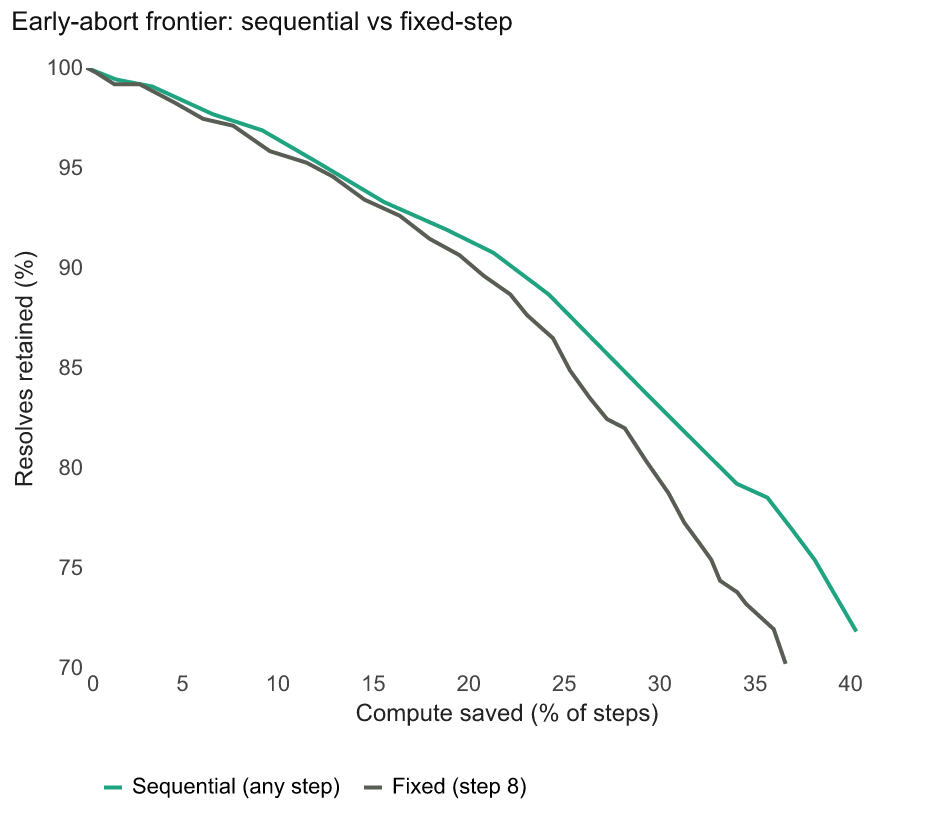
\includegraphics[width=0.7\linewidth]{figures/fig_early_abort_frontier.png}
    \caption{\textcolor{blue}{Early-abort frontier. Re-scoring the prefix at every step and aborting at the first $P(\text{resolve})<\tau$ (sequential, green) trades compute against resolved tasks; sweeping $\tau$ traces the curve. It dominates the best fixed decision step (step 8, grey)---retaining more resolves at any compute budget---and removes the need to choose a decision step. Compute is in canonical action steps.}}
    \label{fig:early_abort}
\end{figure}

\section{Controlled evaluations with procedural controls}
In agent programming and benchmarking, an engineer can specify parameters such as the number of tool use turns and response lengths in the form of tokens, but there is little control over how a task is done. Controlling for behavior at the level of actions is an under-explored way of assessing capabilities---while ablations are possible at different levels of abstraction, it is not possible to say a model can only retrieve context via grep or when, or run a certain number of tests and after what actions.

Fingerprints give us behavioral trends that form the basis for predicting which actions a given agent is most likely to take, useful for next-action prediction and anomaly detection. We batch trajectories into five groups, training models on four and leaving one as a held-out control. As shown in Table~\ref{tab:trajectory_holdouts}, agents fall into three regimes: deterministic scaffolds like Agentless, which are nearly fully predictable (83\% accuracy, $+$50 points over baseline); constrained scaffolds like Moatless, where the scaffold drives behavior and the baseline is already high (68\% accuracy, $+$2 points); and open-ended model-driven agents like Claude and GPT, where predictions are stronger at the single-action level (e.g., Claude-3.5 at 45\% accuracy, $+$27 points). This makes the case for procedural representations as a basis for prediction. We also find that edit streaks are a strong failure signal: for Moatless+DeepSeek-V3, 43\% of trajectories have edit streaks of 5 or more, and of those, the fail rate is 80\%, compared to 59\% for no-streak trajectories. For Claude-3.5 the signal is weaker, with pass rate dropping from 26\% to 11\% with a streak $\geq$5, though the magnitude is comparable.

\begin{table}[H]
\centering\small\setlength{\tabcolsep}{4pt}
\begin{tabular}{lrrrrrr}
\toprule
& \multicolumn{3}{c}{\textbf{Next action}} & \multicolumn{3}{c}{\textbf{Next stage}} \\
\cmidrule(lr){2-4}\cmidrule(lr){5-7}
\textbf{Agent} & Base & Acc. & $\Delta$ & Base & Acc. & $\Delta$ \\
\midrule
\rowcolor{claudebg} Claude-3              & 13\% & 42\% & $+$29 & 33\% & 50\% & $+$17 \\
\rowcolor{claudebg} Claude-3.5            & 18\% & 45\% & $+$27 & 33\% & 52\% & $+$19 \\
\rowcolor{claudebg} Claude-3.7-thinking   & 24\% & 50\% & $+$26 & 33\% & 59\% & $+$26 \\
\rowcolor{claudebg} Claude-4              & 52\% & 58\% & $+$6  & 62\% & 65\% & $+$3  \\
\midrule
\rowcolor{gptbg} GPT-4                 & 21\% & 53\% & $+$32 & 43\% & 65\% & $+$22 \\
\rowcolor{gptbg} GPT-4o                & 27\% & 49\% & $+$22 & 49\% & 62\% & $+$14 \\
\midrule
\rowcolor{owbg} DARS+DeepSeek-R1      & 31\% & 41\% & $+$10 & 37\% & 54\% & $+$17 \\
\rowcolor{owbg} Agentless+Claude-3.5  & 33\% & 83\% & $+$50 & 42\% & 75\% & $+$33 \\
\rowcolor{owbg} Moatless+DeepSeek-V3  & 66\% & 68\% & $+$2  & 66\% & 69\% & $+$3  \\
\bottomrule
\end{tabular}
\caption{Next-action and next-stage prediction accuracy across agent trajectories.}
\label{tab:trajectory_holdouts}
\end{table}

\textcolor{blue}{One application of \texttt{procgrep} is the ability to program and reward model behavior on long-horizon tasks. Typically reward systems for coding models have focused on binary states, but trajectory specifications enable partial rewards based on procedural milestones. A reward spec (YAML) defines phases, penalties, and bonuses over the canonical action sequence:}

\begin{tcolorbox}[colback=black!3, colframe=black!30, boxrule=0.4pt, left=10pt, right=10pt, top=8pt, bottom=8pt, fontupper=\small]
\textcolor{blue}{
\texttt{phases:}\\
\texttt{~~- name: exploration~~~~reward: 0.10}\\
\texttt{~~~~require\_any: [\{action: search\_repo\}, \{action: read\_file\}]}\\
\texttt{~~~~min\_occurrences: 2~~~~before\_first: edit}\\
\texttt{~~- name: implementation~~~~reward: 0.15}\\
\texttt{~~~~require\_any: [\{action: edit\}]}\\
\texttt{~~- name: test\_verification~~~~reward: 0.25}\\
\texttt{~~~~require\_sequence: [edit, run\_test]~~~~max\_gap: 5}\\
\texttt{~~- name: completion~~~~reward: 0.10}\\
\texttt{~~~~require\_any: [\{action: submit\}]}\\
\texttt{penalties:}\\
\texttt{~~- name: edit\_streak~~~~penalty: 0.15}\\
\texttt{~~~~pattern: [edit, edit, edit, edit, edit]~~~~contiguous: true}\\
\texttt{~~- name: no\_search~~~~penalty: 0.05}\\
\texttt{~~~~require\_absent\_before: [search\_repo, read\_file]~~~~before\_first: edit}\\
\texttt{bonuses:}\\
\texttt{~~- name: test\_driven~~~~reward: 0.10}\\
\texttt{~~~~require\_sequence: [run\_test]~~~~before\_first: edit}
}
\end{tcolorbox}

\textcolor{blue}{Scoring a trajectory against this spec returns a structured reward record:}

\begin{tcolorbox}[colback=black!3, colframe=black!30, boxrule=0.4pt, left=10pt, right=10pt, top=8pt, bottom=8pt, fontupper=\small]
\textcolor{blue}{
\texttt{\{"instance\_id": "django\_\_django-12345",}\\
\texttt{~~"binary\_pass": false,~~~~"proc\_score": 0.35,}\\
\texttt{~~"satisfied\_phases": ["exploration", "implementation",}\\
\texttt{~~~~~~~~~~~~~~~~~"test\_verification"],}\\
\texttt{~~"triggered\_penalties": ["edit\_streak"],}\\
\texttt{~~"triggered\_bonuses": []\}}
}
\end{tcolorbox}

\textcolor{blue}{Scoring real trajectories through the spec (\texttt{from procgrep.reward import load\_spec, score}) reproduces a per-agent procedural score across the nine collected agents (Table~\ref{tab:score-vs-heuristic}); a linear scorer over procedures and the library scorer agree to within 0.01, and proc\_score separates resolved from unresolved trajectories by a small margin (corpus $\Delta = +0.03$).} \textcolor{purple}{TODO: re-score the distilled child against this spec once the SWE-agent-LM-32B rollout runs; the prior child 0.795 / teacher 0.940 / 87.8\%-\texttt{stuck\_reading} figures came from an unreconciled spec and an un-run child pipeline, so they are removed pending that run.}

\begin{table}[H]
  \centering
  \begin{tabular}{lccc}
    \toprule
    Agent & Library \texttt{score()} & Inline heuristic & $\Delta$ \\
    \midrule
    Agentless+Claude-3.5 & 0.600 & 0.600 & $0.000$ \\
    DARS+R1              & 0.468 & 0.478 & $-0.010$ \\
    Claude-3.5           & 0.447 & 0.453 & $-0.006$ \\
    Claude-3.7-thinking  & 0.397 & 0.400 & $-0.003$ \\
    Claude-3             & 0.384 & 0.387 & $-0.003$ \\
    GPT-4o               & 0.383 & 0.387 & $-0.004$ \\
    GPT-4                & 0.381 & 0.386 & $-0.005$ \\
    Claude-4             & 0.345 & 0.345 & $0.000$ \\
    Moatless+V3          & 0.187 & 0.191 & $-0.004$ \\
    \midrule
    ALL                  & 0.399 & 0.403 & $-0.004$ \\
    \bottomrule
  \end{tabular}
  \caption{\textcolor{blue}{Per-agent procedural score from the library scorer vs.\ an inline reference heuristic ($\Delta = \text{library} - \text{inline}$); they agree to within 0.01, confirming the spec is reproduced by \texttt{procgrep.reward.score}. proc\_score is a within-scaffold procedural-style measure: \texttt{test\_verification} under-counts shell-invoked test runs (a canonicalization limitation), so it is not a cross-agent capability ranking.}}
  \label{tab:score-vs-heuristic}
\end{table}

\section{Do students behave like their teachers? (a distilled model case study)}
\label{sec:distillation}
\textcolor{blue}{SWE-agent-LM-32B is produced by the SWE-smith pipeline \cite{yang2025swesmith}: Claude-3.7~Sonnet (the teacher) generates SWE-agent trajectories, passing ones are filtered as supervised demonstrations, and Qwen2.5-32B is fine-tuned on the result. Supervision is on \emph{outputs only}---the student reproduces the teacher's actions, not the reasoning behind them. We compare 284 teacher trajectories (Claude-3.7~Sonnet under SWE-agent, on SWE-bench Lite) against 499 child trajectories (SWE-agent-LM-32B, from its public SWE-bench Verified submission); the two pools overlap on 86 shared instances. Because \texttt{lineage\_diff} compares the trajectory \emph{distributions} (vocabulary, entropy, conditional structure) rather than pairing per task, it characterizes teacher-vs-student behavior at the population level---we note the differing task pools as a confound. We measure four axes: vocabulary preservation, entropy shift, outcome-stratified overlap, and conditional structure drift.}

\textcolor{blue}{\textbf{Vocabulary transfers; the distribution concentrates.} The child inherits the teacher's coarse action vocabulary completely (canonical Jaccard $=1.00$) and most of the fine-grained native vocabulary (Jaccard $=0.88$). Yet its per-trajectory action distribution is markedly more concentrated: mean entropy falls from 2.28 to 1.87 bits at the canonical level ($-0.41$) and 2.89 to 2.30 at the native level ($-0.59$). Output-only SFT filtered for the teacher's \emph{passing} trajectories, and the child over-learned that focus into rigidity (Figure~\ref{fig:distillation}a).}

\textcolor{blue}{\textbf{But the drift is neither outcome-dependent nor localized.} We find no support for the intuition that successful child runs are more teacher-like: a child trajectory's native-vocabulary overlap with the teacher is identical whether it resolves the task or not (median Jaccard $0.195$ vs.\ $0.195$). And conditional divergence---how differently the child continues after a given action---is modest and spread across action types (frequency-weighted canonical JSD $\approx 0.05$ over \texttt{edit}, \texttt{read\_file}, \texttt{run\_test}; Figure~\ref{fig:distillation}b), not concentrated at any single decision point. So distillation here transfers the teacher's vocabulary and induces a broad concentration (rigidity), rather than selectively shedding the teacher's decision structure.}

\begin{figure}[H]
\centering
\begin{subfigure}[t]{0.46\linewidth}
    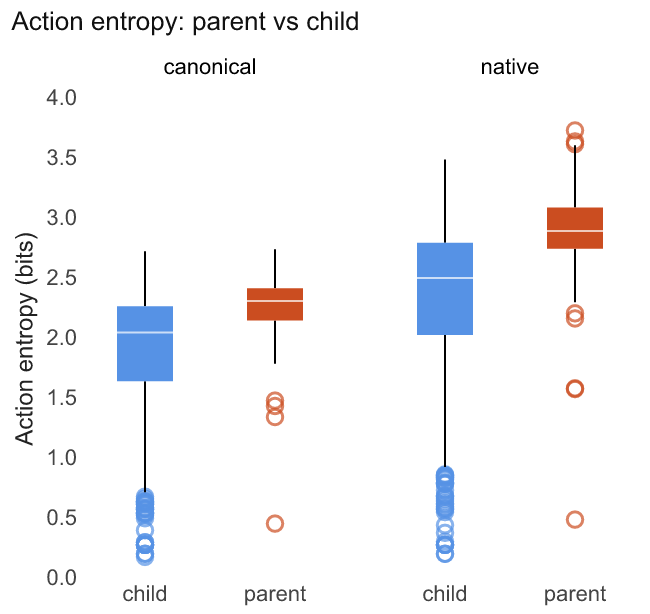
\includegraphics[width=\linewidth]{figures/fig_distillation_A_entropy.png}
    \caption{\textcolor{blue}{Action entropy, teacher vs.\ child (canonical and native). The child distribution is more concentrated ($-0.41$/$-0.59$ bits).}}
    \label{fig:dist_entropy}
\end{subfigure}\hfill
\begin{subfigure}[t]{0.46\linewidth}
    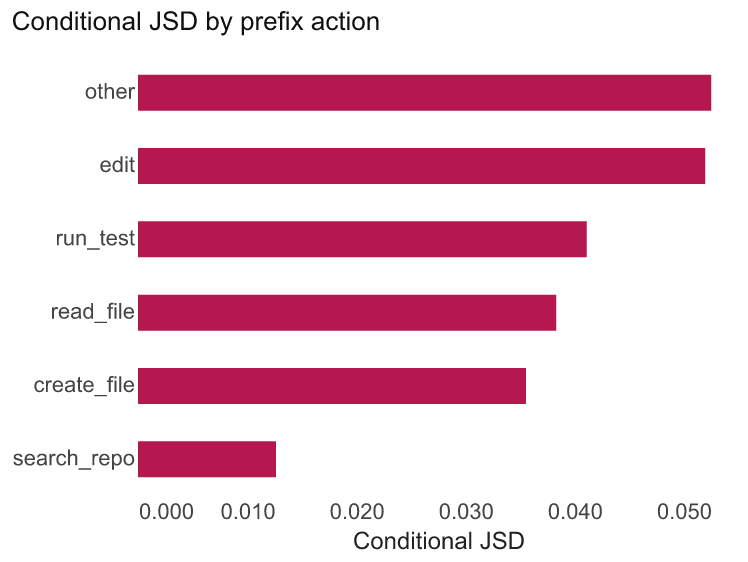
\includegraphics[width=\linewidth]{figures/fig_distillation_B_conditional.png}
    \caption{\textcolor{blue}{Conditional JSD by prefix action (canonical). Divergence is modest and spread, not localized to one control point.}}
    \label{fig:dist_conditional}
\end{subfigure}
\caption{\textcolor{blue}{Distillation: Claude-3.7~Sonnet (teacher, SWE-bench Lite) $\to$ SWE-agent-LM-32B (child, SWE-bench Verified). Vocabulary is preserved (canonical Jaccard 1.0) but the child's action distribution concentrates; the divergence is not outcome-dependent (resolved vs.\ unresolved native Jaccard 0.195 vs.\ 0.195, stated in text) and not localized.}}
\label{fig:distillation}
\end{figure}

\section{Future work}
\textcolor{blue}{Prior work on behavioral diffing and model-diffing has compared model outputs at the response level. Three directions follow from this work. First, \emph{lineage attribution at scale}: applying \texttt{lineage\_diff} across pairs of open-weight models on HuggingFace to ask whether procedural fingerprints can identify training relationships when the relationship is not disclosed. Second, \emph{procedural regression detection} across model releases---the Claude-3.7$\to$Claude-4 opening-move shift (JSD\,=\,0.27 at step~1) shows that training-recipe changes surface as procedural discontinuities. Third, correlating procedural axes with model attributes through observational regression; this can generate hypotheses for controlled distillation experiments like the one in \S\ref{sec:distillation}.}

\section{Appendix}

\begin{figure}[H]
    \centering
    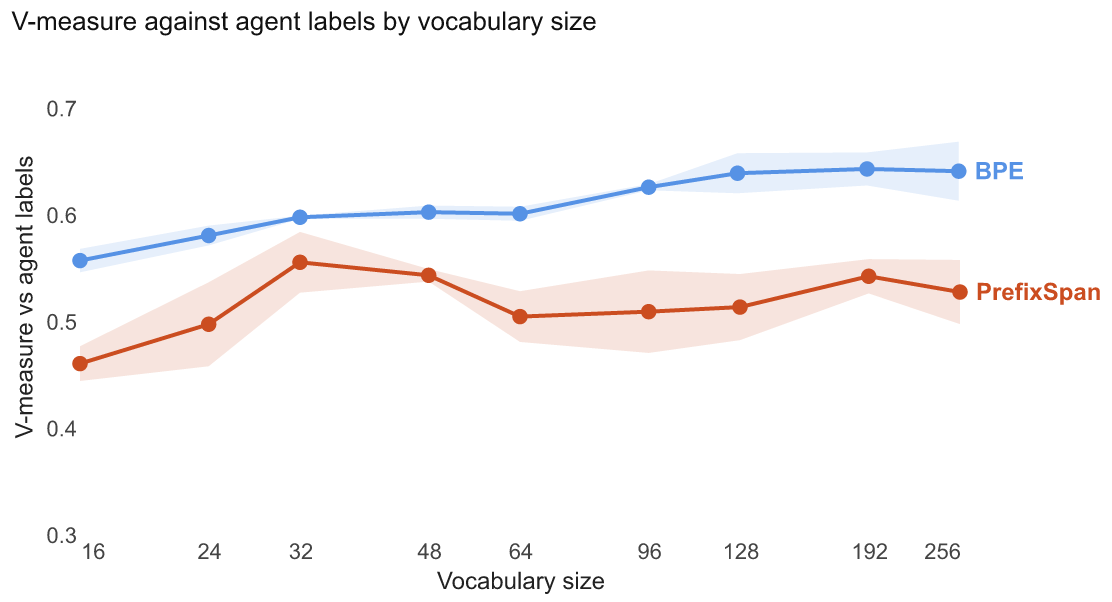
\includegraphics[width=0.6\linewidth]{figures/fig_bpe_vs_prefixspan.png}
    \caption{\textcolor{blue}{Vocabulary induction: BPE separates agents better than PrefixSpan (V-measure against agent labels at matched procedure count).}}
    \label{fig:bpe_vs_prefixspan}
\end{figure}

\begin{figure}[H]
    \centering
    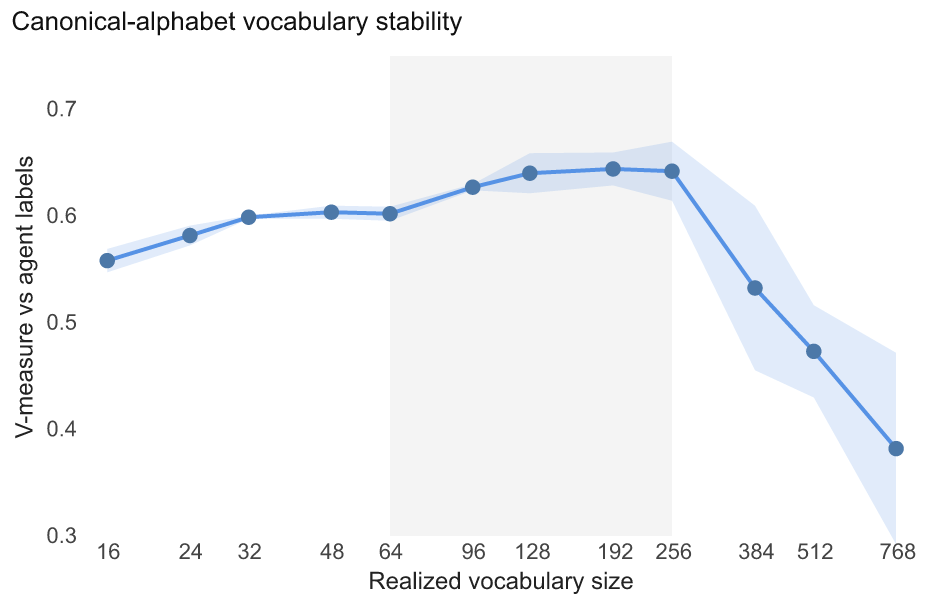
\includegraphics[width=0.6\linewidth]{figures/fig_vmeasure_sweep.png}
    \caption{\textcolor{blue}{V-measure of BPE canonical-vocabulary clustering against agent labels versus realized vocabulary size (5-seed KMeans mean $\pm$ sd). The score rises to a broad plateau of 0.60--0.64 across $V\approx96$--$256$ (high point ${\approx}0.64$ at $V=128$--$192$), then degrades steadily past 256 (0.53 at 384, 0.47 at 512, 0.38 at 768) with sharply rising seed variance as the vocabulary fragments---justifying the $V=64$--$256$ range used throughout (shaded). The plateau, not a sharp peak, is the point: the criterion is robust to vocabulary choice across a wide band.}}
    \label{fig:vmeasure}
\end{figure}

\begin{figure}[H]
    \centering
    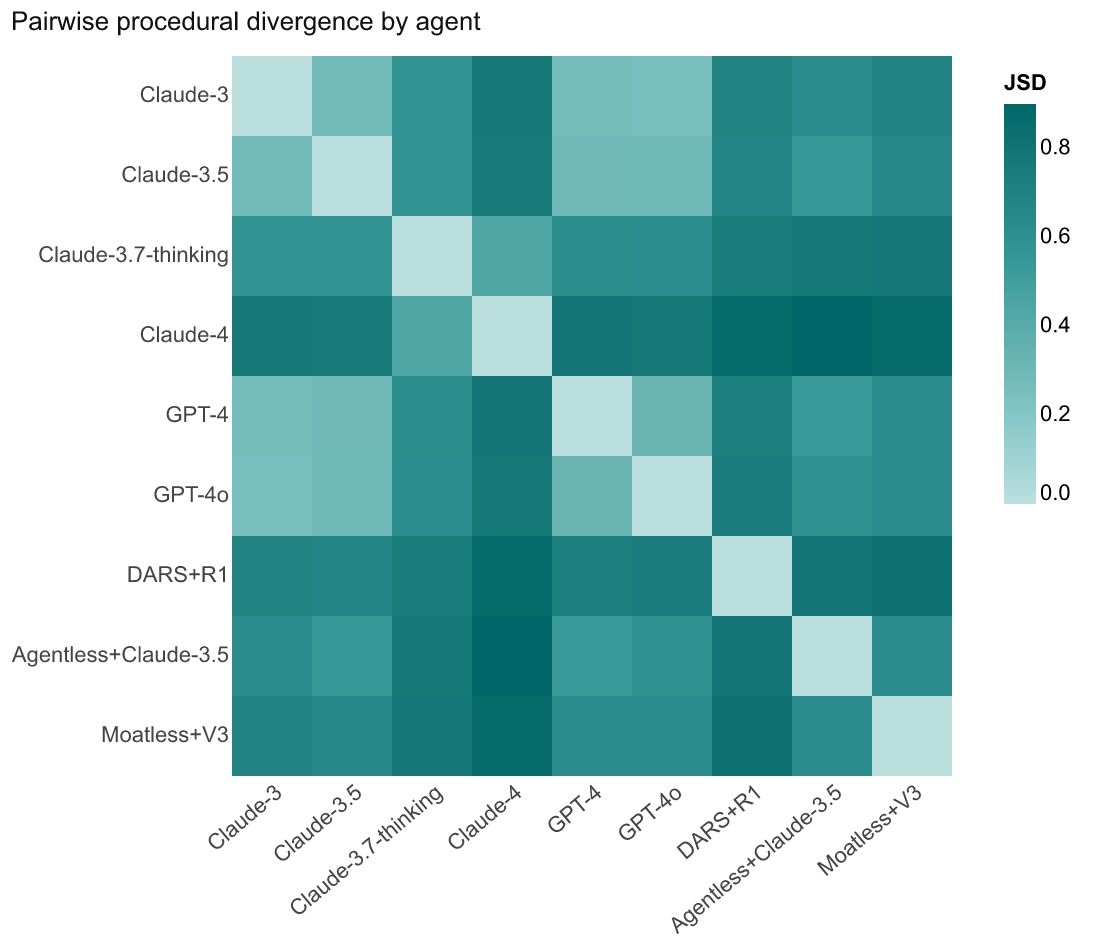
\includegraphics[width=0.9\linewidth]{figures/fig_jsd_matrix_full_canonical.png}
    \caption{\textcolor{blue}{Pairwise JSD between 10 agents at canonical alphabet, grouped by model family and scaffold. The distilled child (SWE-agent-LM-32B) is closest to its parent (Claude-3.7~Sonnet) at JSD\,=\,0.10. The same model under two harnesses diverges at JSD\,=\,0.49, confirming scaffold\,$>$\,era\,$>$\,lineage in procedural impact.}}
    \label{fig:jsd_full}
\end{figure}

\begin{table}[H]
\centering
\begin{tabular}{lcccc}
\toprule
\textbf{Judge model} & \textbf{n} & \textbf{F1 (k=1)} & \textbf{\% compositional} & \textbf{Mean $\kappa$} \\
\midrule
GPT-4o         & 286 & 0.363 & 38.1\% & 0.136 \\
GPT-4o mini    & 285 & 0.246 & 36.5\% & 0.156 \\
Qwen 2.5 72B   &  87 & 0.167 & 17.2\% & 0.128 \\
Llama 3.3 70B  &  87 & 0.000 & 21.8\% & 0.123 \\
\midrule
Weighted mean  & 745 & 0.253 & -- & -- \\
\bottomrule
\end{tabular}
\caption{\textcolor{blue}{Classification results per judge model. The \textbf{Mean $\kappa$} column is the mean pairwise inter-judge agreement on divergence level; the high same-family pairs (GPT-4o vs.\ GPT-4o mini $\kappa=0.38$, Qwen vs.\ Llama $0.31$) lift it to ${\approx}0.13$, but \emph{cross-family} agreement is near zero ($\kappa<0.05$: e.g.\ GPT-4o vs.\ Llama $0.001$, vs.\ Qwen $0.031$), motivating the structural vocabulary approach.}}
\label{tab:divergence_by_model}
\end{table}

\begin{figure}[H]
    \centering
    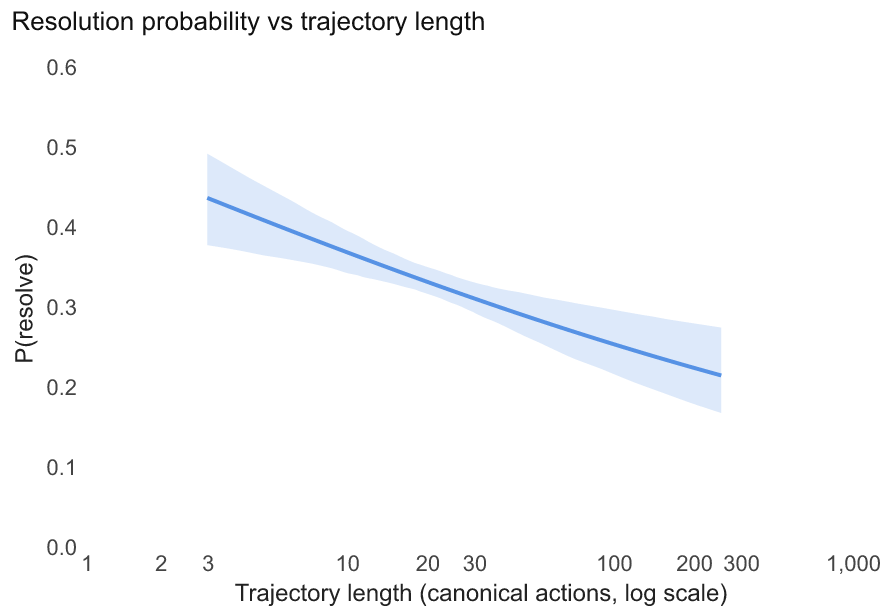
\includegraphics[width=0.85\linewidth]{figures/fig_regression_length.png}
    \caption{\textcolor{blue}{Resolution probability vs.\ trajectory length, logistic fit on $\log_{10}$(length) with a 95\% bootstrap band (length is modeled continuously, not binned). A gentle monotone decline---$P(\text{resolve})$ falls from ${\sim}0.37$ at length 10 to ${\sim}0.28$ at length 60 (log-odds slope $-0.54$ per decade). Length is weakly, not strongly, predictive of failure (consistent with near-equal median lengths of resolved vs.\ unresolved trajectories, 19 vs.\ 20).}}
    \label{fig:regression_length}
\end{figure}

\begin{figure}[H]
    \centering
    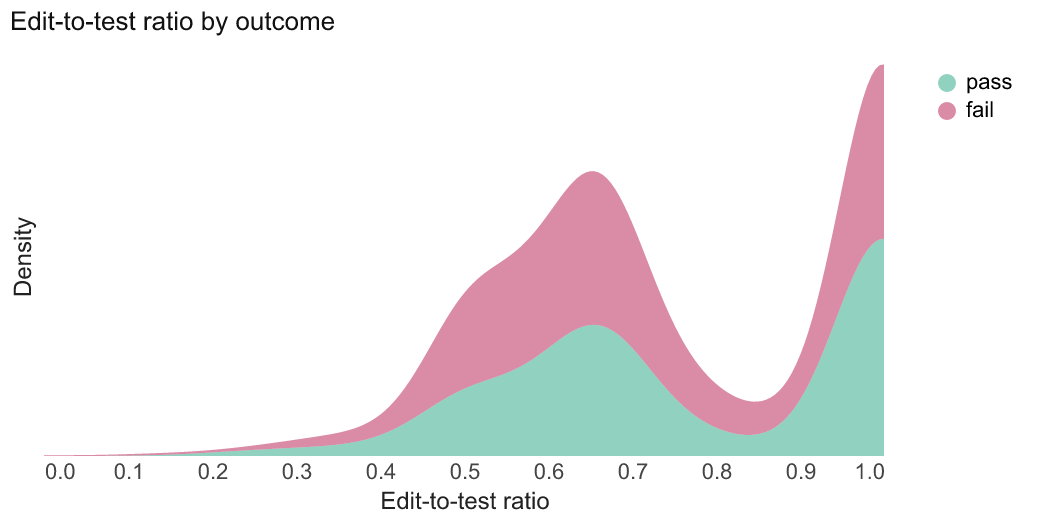
\includegraphics[width=0.85\linewidth]{figures/fig_regression_edit_test.png}
    \caption{\textcolor{blue}{Edit-to-test ratio by outcome. Failing trajectories carry a higher share of test/run actions (median edit-ratio 0.67 vs 0.79 for passing), consistent with unproductive test-thrashing.}}
    \label{fig:regression_edit_test}
\end{figure}


\textcolor{purple}{TODO: Add harness decomposition result as a paragraph or table --- scaffold (JSD 0.49) > model era (JSD 0.36) > training lineage (JSD 0.15).}

\subsection{\textcolor{blue}{Corpus and canonicalization}}
\textcolor{blue}{We study 2{,}639 trajectories from nine agents (Table~\ref{tab:models}) on SWE-bench Lite, plus 499 SWE-agent-LM-32B child trajectories (\S\ref{sec:distillation}) on SWE-bench Verified, all from public leaderboard submissions (\texttt{princeton-nlp/SWE-bench-experiments}; raw trajectories from the submission S3 bucket). Each \texttt{.traj} is mapped to a canonical action sequence by \texttt{canonicalize\_envelope}, which dispatches on scaffold format (SWE-agent, Agentless, DARS, Moatless) and emits a shared ${\approx}76$-atom alphabet. Atoms carry a coarse verb and a file-type tag (e.g.\ \texttt{EDIT\_SRC\_PY}, \texttt{RUN\_PYTHON\_TEST\_PY}, \texttt{OPEN\_SRC\_PY}); chained shell commands are parsed past \texttt{cd\,\&\&} prefixes; Claude-3.7's \texttt{str\_replace\_editor} calls are rewritten into the SWE-agent alphabet; a thought with no tool call emits \texttt{THINK}; unmapped scaffold-specific actions collapse to \texttt{OTHER}. A coarse seven-type projection (\texttt{to\_canon}: \texttt{edit}, \texttt{create\_file}, \texttt{run\_test}, \texttt{read\_file}, \texttt{search\_repo}, \texttt{submit}, \texttt{other}) is used wherever a scaffold-agnostic alphabet is needed (attribution, reward, early-abort).}

\subsection{\textcolor{blue}{Vocabulary induction}}
\textcolor{blue}{Recurring procedures are induced by byte-pair encoding over the canonical sequences. Vocabulary size is selected by a clustering criterion: trajectories are represented as procedure-frequency vectors, clustered with KMeans ($k=$ the number of agents), and scored against agent labels with V-measure (harmonic mean of homogeneity and completeness). Canonical V-measure (5-seed mean) rises to a plateau across $V\approx96$--$256$ and degrades past it as the vocabulary fragments (Figure~\ref{fig:vmeasure}); we use $V$ in the 64--256 range throughout.}

\subsection{\textcolor{blue}{Probe specifications}}
\textcolor{blue}{\emph{Attribution} (Table~\ref{tab:attribution}): TF-IDF over BPE procedures (token pattern \texttt{\textbackslash S+} to keep multi-action procedures intact, unigrams), multinomial logistic regression ($C{=}1$, \texttt{max\_iter}=1000, seed 42), evaluated out-of-fold under \texttt{GroupKFold}($k{=}5$) grouped by task instance; baselines are majority-class, stratified-random, and chance ($1/9$), with a standard-CV comparison as the leakage check. \emph{Early-abort} (Figure~\ref{fig:early_abort}): TF-IDF over unigram+bigram of the first $k$ coarse actions, the same LR and GroupKFold; the sequential policy re-scores every prefix length and aborts at the first $P(\text{resolve})<\tau$; compute is counted in canonical action steps. \emph{Next-action / next-stage} (Table~\ref{tab:trajectory_holdouts}): trajectories split into five groups, leave-one-group-out.}

\subsection{\textcolor{blue}{Reward specification and scorer}}
\textcolor{blue}{The reward spec defines phases, penalties, and bonuses over the coarse action sequence. The library scorer \texttt{procgrep.reward.score} evaluates each rule as a binary match (\texttt{require\_any} with a minimum occurrence count, \texttt{require\_sequence} within a maximum gap, contiguous patterns, and \texttt{before\_first}/\texttt{require\_absent\_before} scoping); satisfied phases and bonuses add their weight, triggered penalties subtract, and the total is clamped to $[0,1]$. The reported per-agent scores (Table~\ref{tab:score-vs-heuristic}) agree with an independent inline reference to within 0.01.}

\subsection{\textcolor{blue}{Narration coverage and verbosity}}
\textcolor{blue}{Forward coverage (does the stated plan cover the actions taken) and reverse coverage (does the account mention each action taken) are computed by aligning the stated action set against the observed canonical action set per trajectory; verbosity is the ratio of stated to observed actions, with a shuffled-rationale control as baseline (Table~\ref{tab:verbosity}, Figure~\ref{fig:cot_alignment}).}

\subsection{\textcolor{blue}{Cost methodology}}
\textcolor{blue}{Token, API-call, and dollar costs are read from \texttt{info.model\_stats} in the raw trajectories (tokens sent/received, API calls, instance cost). Cost telemetry is present only for the SWE-agent submissions; for agents without it, cost-per-step is estimated from published per-token pricing and flagged ($^*$) in Table~\ref{tab:per-agent-megatable}, and the cost panel of Figure~\ref{fig:token_cost_difficulty} is restricted to the cost-available subset.}

\subsection{\textcolor{blue}{Reproducibility}}
\textcolor{blue}{Data sources: SWE-bench Lite leaderboard submissions for the nine agents and the SWE-bench Verified SWE-agent-LM-32B submission for the child trajectories (\texttt{princeton-nlp/SWE-bench-experiments}; trajectories from the public \texttt{swe-bench-submissions} S3 bucket), and \texttt{SWE-bench/SWE-smith-trajectories} on HuggingFace. Probes use seed 42 and scikit-learn defaults except where noted. Analysis scripts are in \texttt{scripts/agent\_trajectories\_paper/}; the canonicalizer, BPE, JSD, \texttt{lineage\_diff}, and reward modules are in the \texttt{procgrep} library.}

\bibliography{main}
\bibliographystyle{apalike}
\end{document}
